\section{Appendix A}
\label{Appendix_A}

\subsection{Defining the Power Spectrum}

Let the function $f(\theta,\phi)$ represent the distribution of the
photo-electrons (PE) on the detector surface. The function
$f(\theta,\phi)$ can be decomposed into a sum of spherical harmonics:

\begin{eqnarray}
\label{eq1}
f(\theta,\phi) = \sum_{\ell=0}^{\infty} \sum_{m=-\ell}^{\ell} f_{\ell m} Y_{\ell m}(\theta,\phi),
\end{eqnarray}

where $Y_{\ell m}$ are Laplace's spherical harmonics defined in a
real-value basis using Legendre polynomials $P_{\ell}$~\cite{legendre_polynomials}:

\begin{eqnarray}
\label{eq2}
Y_{\ell m} = \left\{
  \begin{array}{@{}ll@{}}
    \sqrt{2}N_{\ell m}P_{\ell}^m(\cos\theta)\cos~m\phi, & \text{if}\ m>0 \\
    N_{\ell m} = \sqrt{\frac{(2\ell+1)}{4\pi} \frac{(\ell-m)!}{(\ell+m)!}}, & \text{if}\ m=0 \\
    \sqrt{2}N_{\ell |m|}P_{\ell}^{|m|}(\cos\theta)\sin~|m|\phi, & \text{if}\ m<0
  \end{array}\right.
\end{eqnarray}

where the coefficients $f_{\ell m}$ are defined as
 
\begin{eqnarray}
\label{eq3}
f_{\ell m} = \int_{0}^{2\pi} d\phi \int_0^{\pi} d\theta \sin\theta f(\theta,\phi) Y_{\ell m}(\theta,\phi).
\end{eqnarray}

Equation~\ref{eq4} defines the power spectrum of $f(\theta,\phi)$ in
the spherical harmonics representation, $s_{\ell}$, where $l$ is a multipole
moment. The power spectrum, $s_{\ell}$, is invariant under rotation. 
%It is
%unique to each of the functions $f_i(\theta,\phi)$, $i=$1,2,3...,
%which cannot be transformed into each other by rotation.

\begin{eqnarray}
\label{eq4}
s_{\ell} = \sum_{m=-\ell}^{m=\ell} |f_{\ell m}|^2
\end{eqnarray}

The event topology in a spherical detector determines the distribution
of the PE's on the detector sphere, and, therefore, a set of
$s_{\ell}$'s. These values can serve as a quantitative figure of merit for
different event topologies. The rotation invariance of the $s_{\ell}$'s ensures
that this figure of merit does not depend on the orientation of the
event with respect to the chosen coordinate frame.

The sum of $s_{\ell}$'s over all multipole moments equals to the $L^2$ norm of the
function $f(\theta,\phi)$:

\begin{eqnarray}
\label{eq5}
\sum_{\ell=0}^{\infty} s_{\ell} = \int_{\Omega} |f(\theta,\phi)|^2 d\Omega.
\end{eqnarray}

The normalized power spectrum is thus:

\begin{eqnarray}
\label{eq6}
\mathcal{S}_{\ell} = \frac{s_{\ell}}{\sum_{\ell=0}^{\infty} s_{\ell}} =  \frac{s_{\ell}}{\int_{\Omega} |f(\theta,\phi)|^2 d\Omega},
\end{eqnarray}

and can be used to compare the shapes of various functions
$f(\theta,\phi)$ with different normalizations. As the total number of
PEs detected on the detector sphere fluctuates from event to event we
use the normalized power $\mathcal{S}_{\ell}$.


\subsection{Spherical Harmonics Analysis and Off-center Events}

In general, events with the same event topology result in the same
the power spectrum $S_{\ell}$ only if events originate in the center 
of the detector. In
order to compare the spherical harmonics for events with verticies away
from the center, a coordinate transformation for each photon hit is
needed. The necessary transformation applied for each PE within an
event is illustrated in Fig.~\ref{fig:SphH_transform}.  The solid
circle in Fig.~\ref{fig:SphH_transform}~has a radius R and shows the
actual detector boundaries. The dotted circle shows a new sphere with
the same radius R, which now has the event vertex in its center. The
radius vector of each PE is stretched or shortened to its intersection
with this new sphere using the transformation, $\vec{r}^{,}_{PE} =
\frac{\vec{a}}{|\vec{a}|} \cdot R$, where $\vec{r}^{,}_{PE}$ is a new
radius vector of a PE and $\vec{a}=\vec{r}_{PE} - \vec{r}_{vtx}$ with
$\vec{r}_{PE}$ and $\vec{r}_{vtx}$ being radius vectors of the PE and
the vertex in the original coordinates, respectively.

\begin{figure*}[h]
  \centering
%  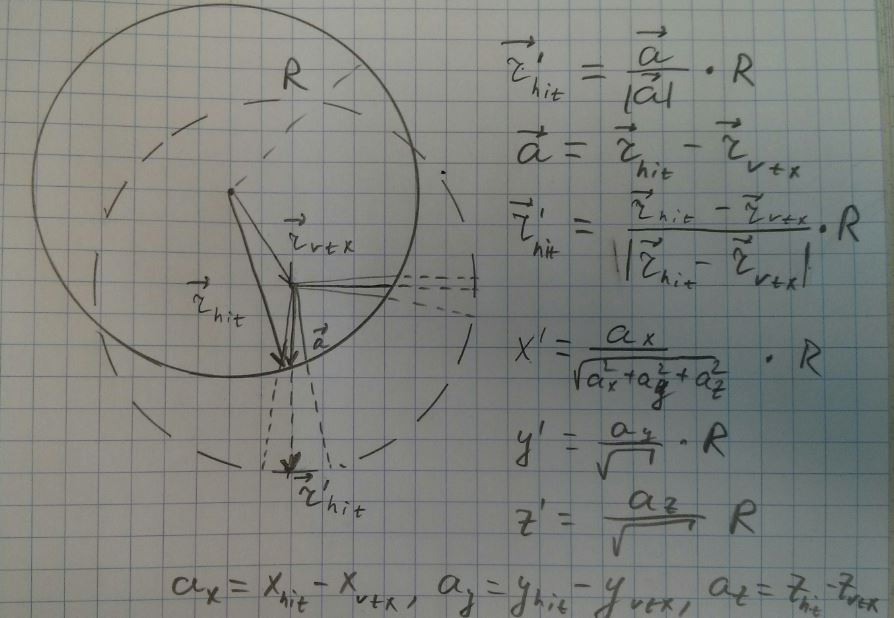
\includegraphics[width=0.95\textwidth]{SphH_transform_sketch.JPG}
  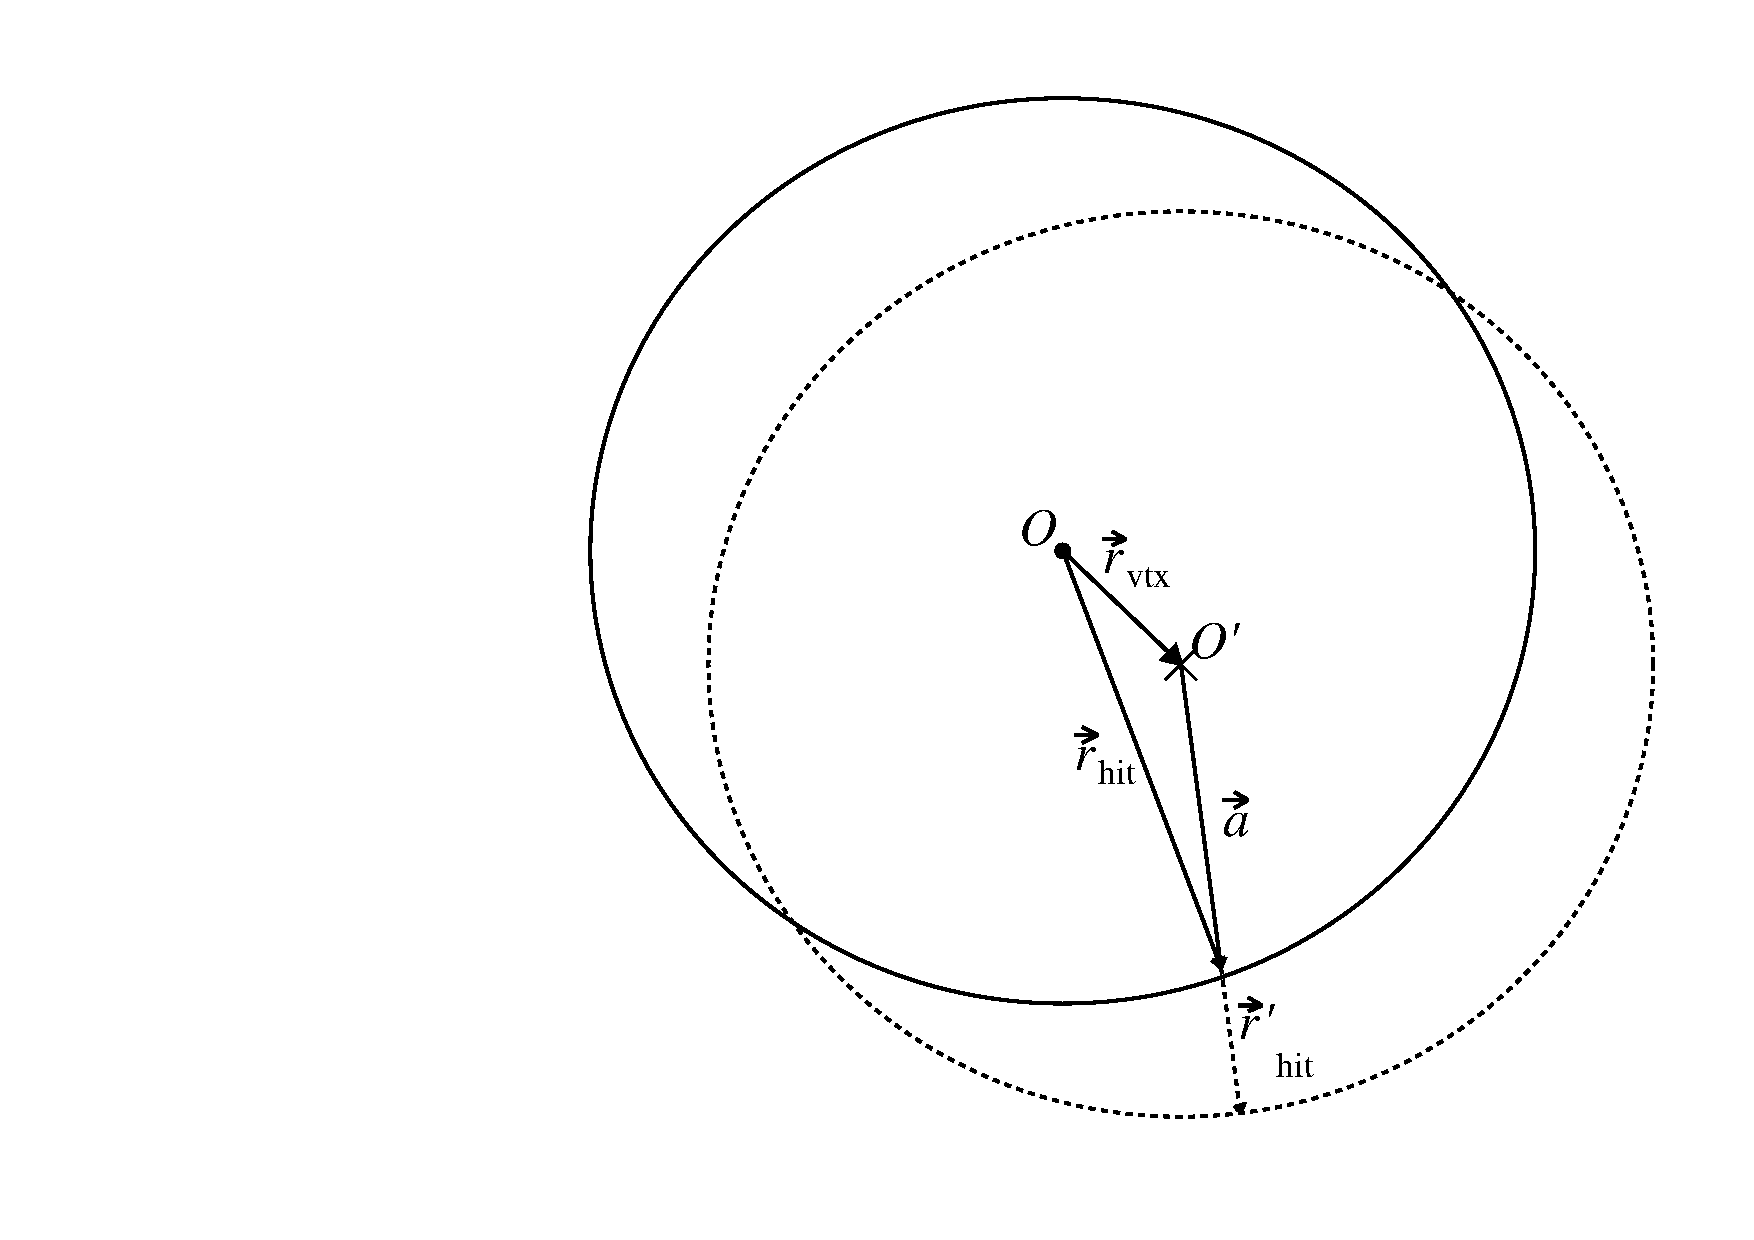
\includegraphics[width=0.4\textwidth]{SphH_transform.pdf}
  \caption{The coordinate transformation which is applied to events that are
    off-center. The solid circle schematically shows the actual detector
    boundaries. The dotted circle shows a new sphere of radius R$=$6.5~m
    with the event vertex position in the center. The radius vector of
    each photon hit is stretched or shortened until the intersection with
    this new sphere using the transformation $\vec{r}^{,}_{hit} =
    \frac{\vec{a}}{|\vec{a}|} \cdot R$, where $\vec{r}^{,}_{hit}$ is a
    new radius vector of the photon hit, $R$ is detector sphere radius,
    and $\vec{a}=\vec{r}_{hit} - \vec{r}_{vtx}$ with $\vec{r}_{hit}$
    and $\vec{r}_{vtx}$ being the radius vectors of the photon hit and
    vertex position in original coordinates, respectively.}
  \label{fig:SphH_transform}
\end{figure*}


%\subsection{Implementation of the spherical harmonics analysis}

%The numerical calculation of the power spectrum is implemented as follows.
%For each event, a 2-D histogram of  the distribution of PEs on the
%detector surface in $\theta$ vs $\phi$ is created. We then treat this
%histogram as a function $f(\theta,\phi)$, where the value of the
%function for any pair of $\theta$ and $\phi$ is equal to the number of
%PE's in the histogram bin corresponding to that pair.

%The coefficients $f_{\ell m}$ from Eq.~\ref{eq3} are calculated using a
%Monte Carlo integration technique. The values of the $S_{\ell}$ moments are
%calculated using Eqs.\ref{eq4} - \ref{eq6}. 
%{\bf Also need to provide
%reference to the libraries for Legendre polynomials.}


